%!TEX root = ../thesis.tex
\begin{savequote}[75mm]
	A goal without a plan is just a wish.
%\qauthor{Quoteauthor Lastname}
\end{savequote}

\chapter{The project}
\label{chapter_2}

This chapter contains the results of the discussions and planning that have been made prior to the beginning of the internship.
These contents are described in more detail in the \Quote{Piano di Lavoro} (work plan in English), a document that contains an estimation of resources for each task that composes the project.
\Chapref{AppendixA} contains two extracts from that document: a table with the hours spent per task and a Gantt chart.
For both it's present the original estimation and a final version.\\
At the beginning of May there was a first meeting with the tutor to understand the needs of the company and draft a plan.
Below follows a description about the project and how it was approached.

\section{The company's needs}
	At the time of writing it has nearly 40 employees and it is expected to hire new people soon.\\
	Athonet uses multiple software tools for keeping track of projects, sharing information internally and with the clients, visualizing \gls{product roadmaps}\glsadd{Roadmap}, etc.\\
	The most important tools they are currently relying on are:
	\begin{itemize}
		\item \Quote{Redmine}\cite{redmine} as an Issue Tracking System
		\item \Quote{SharePoint}\cite{sharepoint} as a collaborative platform
		\item \Quote{Planner}\cite{planner} for visualizing project roadmaps
		\item \Quote{GitLab}\cite{gitlab} as a \gls{repository}\glsadd{Repository}
	\end{itemize}
	While some of these software packages are compatible, others were not developed to be used together, although there are plugins that allow to interconnect them.
	These don't allow much customization since they are programmed by third party developers and not always the compatibility is up to date with the latest releases.\\
	Consequently there is a need to provide employees with a suite of stable tools that are easily interconnected and with a vast and well done documentation.
	Also, these tools must be easy to maintain and update, since they don't have to become obsolete and outdated.\\
	Nobody likes legacy systems.
	\begin{figure}[H]
		\centering
		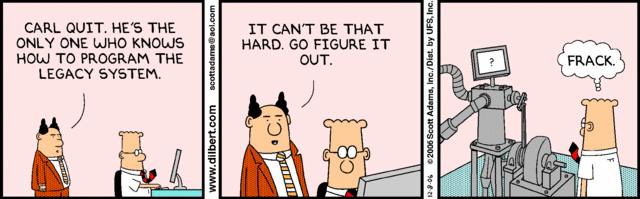
\includegraphics[width=1\textwidth]{resources/legacy-code}\\
		\caption{Dilbert on legacy system infrastructures}
	\end{figure}
	Internal changes may not be directly visible to the clients, but the effect of having a more organized company, where there is always track of the work done and in progress, ensures that when there is a request from the client it does not go unseen or unanswered.\\
	Although, forcing employees to use a software instead of another one is not easy without creating chaos.
	This is why a good and available documentation is the key on helping employees transition from a tool to another.

\section{Requirements and objectives}
	The final objective was to create a suitable and working environment that would be ready to transfer it into production and explain the users how to use it.\\
	Requirements can be divided in three categories based on their relevance:
	\begin{itemize}
		\item Mandatory
		\item Desirable
		\item Optional
	\end{itemize}
	A detailed list of requirements that describe more accurately the ones included in the original planning document can be found in \ref{AppendixB}.
	
\section{Time division and planning}\label{sec:time_planning}
	The time division of the project has been visualized using a Gantt diagram, alongside a table that contains a realistic approximation of the hours spent per task.\\
	The internship was planned for a duration of ten weeks and the project has been spread such that there would be enough time to understand the tools and use them to get acquainted and demo them to the other employees.
	This time period also includes the phases for getting feedback from users, fine tune the configuration, explain the tools to various members of the company and, in case of incidents, slack time.
	The complete Gantt diagram can be found in \ref{gantt_1}.\\
	This temporal sequence has been draft only after understanding the requirements and getting an idea about how Atlassian's software works, also I wanted to perceive the final objective and think on how to achieve it.
	As can be seen in the Gantt diagram, there are some tasks that overlap in time: for example the \Quote{Study of the Atlassian suite} overlaps with Configuration of the environment tools.
	This because the tasks may have something in common or one helps the achievement of the other.
	While studying the requirements for the Atlassian software I decided I would also configure the host machine.\\
	I have coarse grained planned four main time periods: \Quote{Learning}, \Quote{Implementing}, \Quote{Testing and fine tuning}, \Quote{Feedback}.
	Each of these contain smaller tasks that involve studying the tools, installing and configuring them, etc.\\
	As discussed with the tutor, meetings had to be considered so that the progress done could be explained to him and the other company figures that would eventually use the software.\\
	As \gls{milestones}\glsadd{Milestone}, in agreement with the tutor, the deliverable that marks the progress of the work was a VM that represented the status of the system.
	By definition this must be versionable and with a well written changelog.
	